\documentclass[11pt,a4paper]{article}
\usepackage[T1]{fontenc}
\usepackage[utf8]{inputenc}
\usepackage[margin=2.5cm]{geometry}
\usepackage{amsmath,amssymb,booktabs,graphicx,xcolor}
\usepackage[numbers,sort&compress]{natbib}
\usepackage[colorlinks=true,linkcolor=blue!50!black,citecolor=blue!50!black,urlcolor=blue!50!black]{hyperref}
% Generated by make_table.py from ../output/design_scan.csv
\newcommand{\resPhiZero}{1.95}
\newcommand{\resAdaptZero}{1.54}
\newcommand{\resbTZero}{1.04}
\newcommand{\respTZero}{1.25}
\newcommand{\resHealthZero}{0.37}
\newcommand{\resMismatchZero}{1.54}
\newcommand{\resPhiOne}{6.59}
\newcommand{\resAdaptOne}{0.26}
\newcommand{\resbTOne}{0.26}
\newcommand{\respTOne}{0.31}
\newcommand{\resHealthOne}{5.58}
\newcommand{\resMismatchOne}{0.79}
\newcommand{\resSolves}{12}
\newcommand{\resConverged}{8}

\newcommand{\R}{\mathbb{R}}

\title{Control of adaptation: steering an adaptive body with a designed adaptive implant\\[0.3em]
\large First report on the co-evolution project}
\author{Sebastian Sager\thanks{Draft prepared with the AI assistant Claude (Anthropic) on
2026-10-05: literature search, model exploration, implementation, and text. All
statements require review by the author.}}
\date{October 5, 2026}

\begin{document}
\maketitle

\begin{abstract}
We consider two adaptive agents, a body and an implant, that adapt to each other until
they reach an equilibrium. The designer can neither act on the body nor prescribe the
implant's actions, but designs the implant's adaptation mechanism, here its objective.
The quality of a design is judged by the equilibrium that the coupled system reaches:
how close the body ends to a desired healthy state and how well the implant is
integrated. We position this \emph{control of adaptation} against the two-learner problem
in neural interfaces, co-adaptation, human-in-the-loop optimization, adaptive and dual
control, learning in games, and strategic delegation. A minimal two-player differential
game with one state, one control, and one objective per player, solved with the
optimal-control based solver CorleoneGame.jl, shows a non-trivial effect: an implant
that pursues exactly the designer's objective is exploited, because the body lets the
implant do the adapting. An implant designed to disregard the mismatch leads the body to
the healthy state and yields a markedly lower designer cost, although the designer
values integration. This is the commitment effect known from strategic delegation,
here in a dynamic co-adaptation game.
\end{abstract}

\section{Question}
An implant (a device, a material, a controller, or a cell therapy) and the body it is
placed in adapt to each other. The body regulates and remodels; the implant changes its
state according to a built-in mechanism. Both processes are goal-directed, and the
outcome of their interplay is an equilibrium of the coupled adaptation. Whether this
equilibrium is close to a desired \emph{healthy} state depends on how the implant adapts.
The design problem is therefore
\begin{equation}\label{eq:design}
\min_{\theta\in\Theta}\ \Phi\bigl(x^\ast(\theta)\bigr)\quad\text{s.t.}\quad
x^\ast(\theta)\ \text{is an equilibrium of the game between body and implant}(\theta),
\end{equation}
where $\theta$ parametrizes the implant's adaptation mechanism and $\Phi$ measures the
distance of the co-adapted outcome from the healthy state. The designer acts once, before
the interaction, on \emph{how the implant adapts}; it does not adapt a controller to an
unknown plant. We call this \emph{control of adaptation}, in contrast to adaptive control.
The project name uses ``co-evolution''; since evolutionary biology reserves this term for
reciprocal genetic change across generations \citep{DieckmannLaw1996}, ``co-adaptation''
may be the more precise term for publications.

\section{Relation to existing approaches}

\paragraph{Two-learner problem and co-adaptation.}
In brain-machine and body-machine interfaces, user and decoder adapt simultaneously;
this ``tale of two learners'' \citep{PerdikisMillan2020} has been addressed with
co-adaptive decoders \citep{DiGiovanna2009}, by showing that decoder adaptation shapes
neural plasticity \citep{Orsborn2014}, with co-adaptation frameworks \citep{DeSantis2021},
and by tuning decoder learning rates for estimation performance \citep{HsiehShanechi2018}.
Closest to the present question, brain and decoder have been modeled as strategic agents
with own costs whose gradient learning converges to Nash equilibria depending on the
learning rates \citep{Madduri2021}; decoder learning rate and regularization were then
designed to \emph{shape} the co-adaptive outcome \citep{Madduri2024}, and machine learning
algorithms were shown to select among game-theoretic equilibria in experiments with
humans, including steering humans to the machine's optimum \citep{Chasnov2025}.
The idea of designing a machine's adaptation to shape a joint equilibrium is therefore not
new. The present project differs in (A) continuous-time dynamic games with state
dynamics, horizons, and running costs instead of static quadratic games with gradient
learners, (B) designing the implant's objective and adaptation law, judged by a designer
criterion that differs from the implant's own objective, (C) biological implant--body
interactions, and (D) equilibria computed by optimal-control best responses, which admit
nonlinear dynamics and state and path restrictions.

\paragraph{Human-in-the-loop optimization.}
Device parameters are optimized online against a measured human objective, e.g.,
metabolic cost under exoskeleton assistance \citep{Zhang2017}. The human enters as a
black-box objective, not as a modeled strategic agent, and no equilibrium is predicted.

\paragraph{Adaptive and dual control.}
Adaptive control adjusts a controller to a plant with unknown parameters
\citep{AstromWittenmark1995}; dual control adds deliberate probing to learn while
controlling \citep{Feldbaum1960,Wittenmark1995}. In both, the plant is not goal-directed.
Here the plant (body) adapts toward its own goals, and the controller's adaptation law is
the design variable. Dual control becomes relevant when the body's objective is unknown
and the implant must learn it while steering.

\paragraph{Learning in games, opponent shaping, steering, teaching.}
Learning dynamics and their equilibria are the subject of learning in games
\citep{FudenbergLevine1998,Chasnov2020}. Opponent-learning awareness lets an agent shape
the anticipated learning step of the other \citep{Foerster2018}; payments can steer
no-regret learners to a desired equilibrium \citep{ZhangSteering2023}; machine teaching
designs the inputs of a single learner \citep{Zhu2015}. These approaches act during the
learning process; the design considered here acts once on the implant's preferences.

\paragraph{Incentive design and strategic delegation.}
Problem~\eqref{eq:design} is a bilevel problem related to Stackelberg and incentive
design in dynamic games \citep{BasarOlsder1999,HoLuhOlsder1982,Ratliff2019}. Its
designer--implant--body structure is that of strategic delegation: a principal gains by
giving its agent preferences that differ from its own, because the agent's preferences
act as a commitment in the agent's game with a third party
\citep{Vickers1985,FershtmanJudd1987}. The indirect evolutionary approach
\citep{GuthYaari1992} has the same structure, with preferences selected by the material
outcome of equilibrium play. The example below reproduces the delegation effect.

\section{A minimal co-adaptation game}
States $b(t)$ (body) and $p(t)$ (implant) are one-dimensional, e.g., a tissue property
and the corresponding implant setting. Each player owns one control, its adaptation rate:
\begin{align}
\dot b &= u_B\,(p-b), & u_B(t)&\in[0,1], & b(0)&=0,\\
\dot p &= u_P\,(b-p), & u_P(t)&\in[-1,1], & p(0)&=1.
\end{align}
This is the coupled relaxation $\dot b=\alpha(p-b)$, $\dot p=\beta(b-p)$ with the
adaptation rates $\alpha,\beta$ replaced by decisions of the players. The body can only
move toward the implant; the implant can yield to the body ($u_P>0$) or lead away from it
($u_P<0$). The body starts in its diseased state $s=0$; the implant is set to the healthy
state $h=1$ at implantation. On the horizon $[0,T]$, $T=10$, the players minimize
\begin{align}
J_B &= \int_0^T (p-b)^2 + w_s\,(b-s)^2 + c_B\,u_B^2\,dt, \\
J_P^\mu &= \int_0^T \mu\,(p-b)^2 + (b-h)^2 + c_P\,u_P^2\,dt,
\end{align}
with $w_s=0.2$, $c_B=c_P=0.1$. The body dislikes the mismatch with the implant, is
attached to its set point (homeostasis), and pays for plasticity. The implant's objective
is the design: the weight $\mu\ge0$ on the mismatch. The designer values health and
integration equally and accepts the implant's effort,
\begin{equation}
\Phi = \int_0^T (p-b)^2 + (b-h)^2 + c_P\,u_P^2\,dt ,
\end{equation}
so that $\mu=1$ is the \emph{sincere} design: the implant pursues exactly the designer's
objective. Each player has one state, one control, and one objective.

\paragraph{Numerical method.}
For each design $\mu\in\{0,0.1,0.25,0.5,1,2\}$, an open-loop Nash equilibrium candidate is
computed with CorleoneGame.jl (sequential damped best responses, each an optimal control
problem in single shooting with Ipopt; damping $0.2$; at most 300 rounds; 20 and then 40
piecewise-constant control intervals). A candidate is accepted when no player improves its
objective by more than the relative tolerance $2\cdot10^{-5}$ in a deviation audit by local
solves. Since the game may have several equilibria, each design is solved from two initial
policies, $(u_B,u_P)=(0.3,0)$ and $(0.1,1)$. An independent Python prototype (best responses
by L-BFGS-B on 20 intervals, RK4 integration) gave the same values for the designs it
reached: $\Phi=1.963$ (Python, 20 intervals) versus $1.953$ (CorleoneGame, 40 intervals)
for $\mu=0$, and $3.970$ versus $3.970$ for $\mu=0.5$ and $6.12$ versus $6.05$ for $\mu=2$, both
on 20 intervals (\texttt{checks/grid20\_2026-10-05.txt}). Of the \resSolves{} solves, \resConverged{} satisfied the audit tolerance; the
others reached the round limit and are reported but not certified.
The code is \texttt{co-evolution/simple.jl}.

\section{Results}
Figure~\ref{fig:simple} and Table~\ref{tab:scan} summarize the scan.

\begin{figure}[t]
\centering
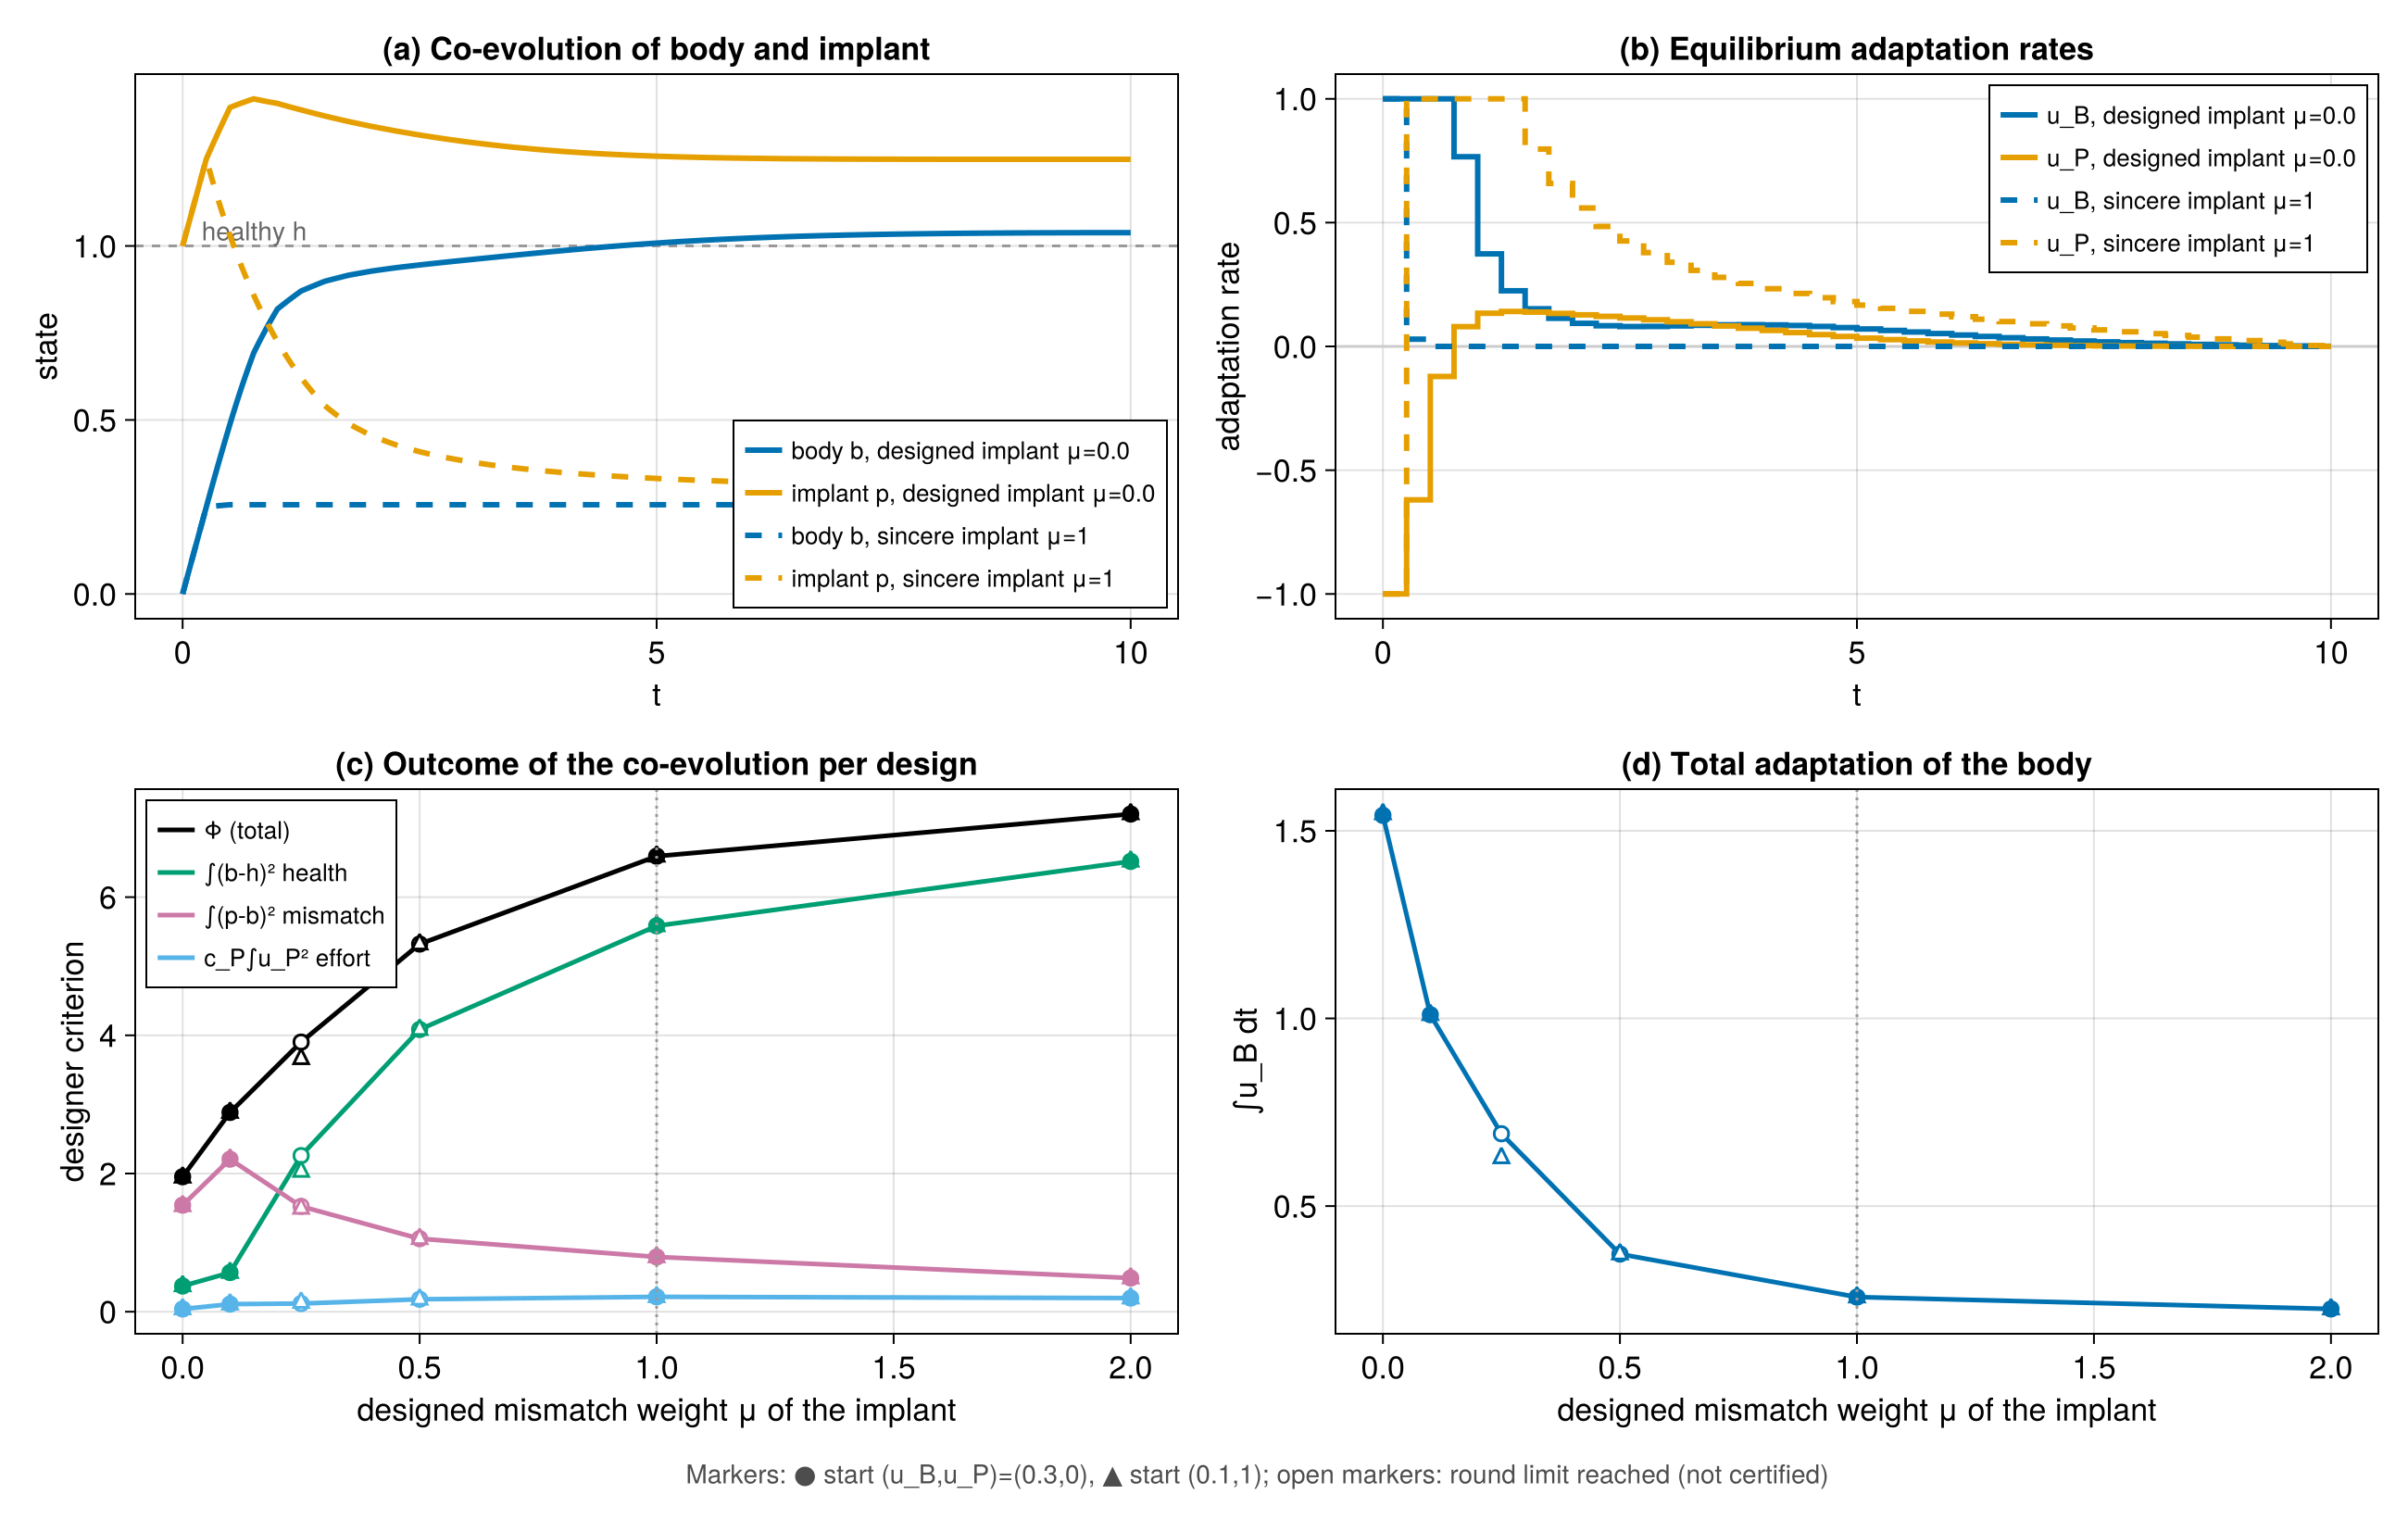
\includegraphics[width=\textwidth]{../output/simple.png}
\caption{(a) Equilibrium trajectories of body $b$ (blue) and implant $p$ (orange) for the
designed implant $\mu=0$ (solid) and the sincere implant $\mu=1$ (dashed); the gray line is the
healthy state. (b) Equilibrium adaptation rates. (c) Designer criterion $\Phi$ and its parts
over the design $\mu$; the dotted line marks the sincere design. (d) Total adaptation
$\int u_B\,dt$ of the body. Lines connect the solves from the start $(0.3,0)$; open markers
indicate solves that reached the round limit.}
\label{fig:simple}
\end{figure}

\begin{table}[t]
\centering\small
% Generated by make_table.py from ../output/design_scan.csv
\begin{tabular}{rlcrrrrrrr}
\toprule
$\mu$ & start $(u_B,u_P)$ & conv. & $\Phi$ & $\int(b-h)^2$ & $\int(p-b)^2$ & $c_P\!\int u_P^2$ & $\int u_B$ & $b(T)$ & $p(T)$\\
\midrule
0 & (0.3, 0) & yes & 1.953 & 0.372 & 1.542 & 0.040 & 1.541 & 1.038 & 1.249\\
0 & (0.1, 1) & yes & 1.946 & 0.374 & 1.532 & 0.040 & 1.545 & 1.036 & 1.244\\
0.1 & (0.3, 0) & yes & 2.884 & 0.567 & 2.208 & 0.110 & 1.010 & 0.868 & 1.049\\
0.1 & (0.1, 1) & yes & 2.883 & 0.566 & 2.207 & 0.110 & 1.010 & 0.868 & 1.049\\
0.25 & (0.3, 0) & no & 3.903 & 2.259 & 1.525 & 0.119 & 0.693 & 0.562 & 0.689\\
0.25 & (0.1, 1) & no & 3.661 & 2.030 & 1.496 & 0.135 & 0.628 & 0.578 & 0.692\\
0.5 & (0.3, 0) & no & 5.321 & 4.084 & 1.057 & 0.180 & 0.372 & 0.370 & 0.442\\
0.5 & (0.1, 1) & no & 5.321 & 4.084 & 1.057 & 0.180 & 0.372 & 0.370 & 0.442\\
1 & (0.3, 0) & yes & 6.593 & 5.585 & 0.793 & 0.216 & 0.257 & 0.256 & 0.308\\
1 & (0.1, 1) & yes & 6.593 & 5.585 & 0.793 & 0.216 & 0.257 & 0.256 & 0.308\\
2 & (0.3, 0) & yes & 7.203 & 6.517 & 0.488 & 0.198 & 0.226 & 0.195 & 0.232\\
2 & (0.1, 1) & yes & 7.205 & 6.520 & 0.488 & 0.198 & 0.226 & 0.195 & 0.232\\
\bottomrule
\end{tabular}

\caption{Design scan. Columns: implant mismatch weight $\mu$, initial policy, audit
passed, designer criterion and its parts, total body adaptation, and terminal states.}
\label{tab:scan}
\end{table}

\paragraph{The sincere implant is exploited.}
With $\mu=1$, the body adapts in one short burst at the start ($u_B=1$ on the first
interval) and then stops, while the implant keeps yielding ($u_P>0$) until the mismatch is
small. In total the body adapts little ($\int u_B\,dt=\resAdaptOne$): it lets the implant do
the adapting.
Both meet far from health, $b(T)=\resbTOne$, $p(T)=\respTOne$, and
$\Phi=\resPhiOne$, dominated by the health term ($\resHealthOne$).

\paragraph{The designed implant leads.}
With $\mu=0$, the implant first leads away from the body ($u_P=-1$ and $u_P\approx-0.6$ on
the first two intervals, $p$ rises to about $1.4$) and afterwards yields only slightly
($u_P\approx0.1$). The body cannot reduce its mismatch cost except by adapting itself and does so
strongly ($\int u_B\,dt=\resAdaptZero$), slightly beyond the healthy state, $b(T)=\resbTZero$, with the implant at
$p(T)=\respTZero$. The designer's cost drops to $\Phi=\resPhiZero$. The mismatch part is
larger than with the sincere implant ($\resMismatchZero$ versus $\resMismatchOne$), but
health improves by far more ($\resHealthZero$ versus $\resHealthOne$).

\paragraph{Interpretation.}
The co-adaptation is a game of who yields. Each agent prefers that the other adapts. An
implant that cares about integration is predictably accommodating, and the body
free-rides on this accommodation. An implant that does not care cannot be exploited; it
commits to its position, and the body's own mismatch aversion makes it follow. The
designer, who does care about integration, achieves more of both health and overall value
by \emph{delegating} to an implant with different preferences. This is the commitment effect of
strategic delegation \citep{Vickers1985,FershtmanJudd1987} in a dynamic co-adaptation
game, and it shows ``adaptive steering of another adaptive system'': the designer steers
the body only through the implant's adaptation mechanism.

\paragraph{Limitations.}
(A) The equilibria are open-loop and computed by local solves; the audit does not prove
global Nash optimality. The two initial policies gave the same candidates up to small differences
($|\Delta\Phi|\le0.01$), except for the uncertified $\mu=0.25$, but the control grid matters: on 20 intervals, the designs $\mu=0.5$ and $\mu=2$
reached certified candidates with $\Phi=3.97$ and $6.05$, on 40 intervals uncertified $5.32$
and certified $7.20$ (Table~\ref{tab:scan}). This indicates several equilibria or a
grid-dependent equilibrium selection. All values for $\mu>0$ remain far above $\Phi$ at
$\mu=0$, so the main conclusion does not depend on this. (B) Intermediate designs, notably $\mu=0.25$, did not
converge within the round limit; their values are not certified. (C) One parameter set; the
optimum at the boundary $\mu=0$ may change for other parameters, e.g., a stronger
homeostatic attachment $w_s$. (D) The body's objective is assumed known to the designer.
(E) The model is a caricature without calibrated biology.

\section{Next steps}
The editable list is \texttt{co-evolution/nextsteps.md}. In brief:
(A) consolidate the example (finer design grid, second design variable $p(0)$,
robustness against a misspecified body, comparison with the Stackelberg design);
(B) richer implant mechanisms: parametrized adaptation laws, feedback policies, and
learning-rate designs as in \citep{Madduri2024};
(C) biologically grounded instances, e.g., bone remodeling with stress shielding,
closed-loop neuromodulation, or tolerance constraints (rejection when the mismatch is too
large); (D) unknown body: inverse games and dual control.

\bibliographystyle{plainnat}
\bibliography{coevolution}
\end{document}
